\begin{figure}[t]
    \centering
    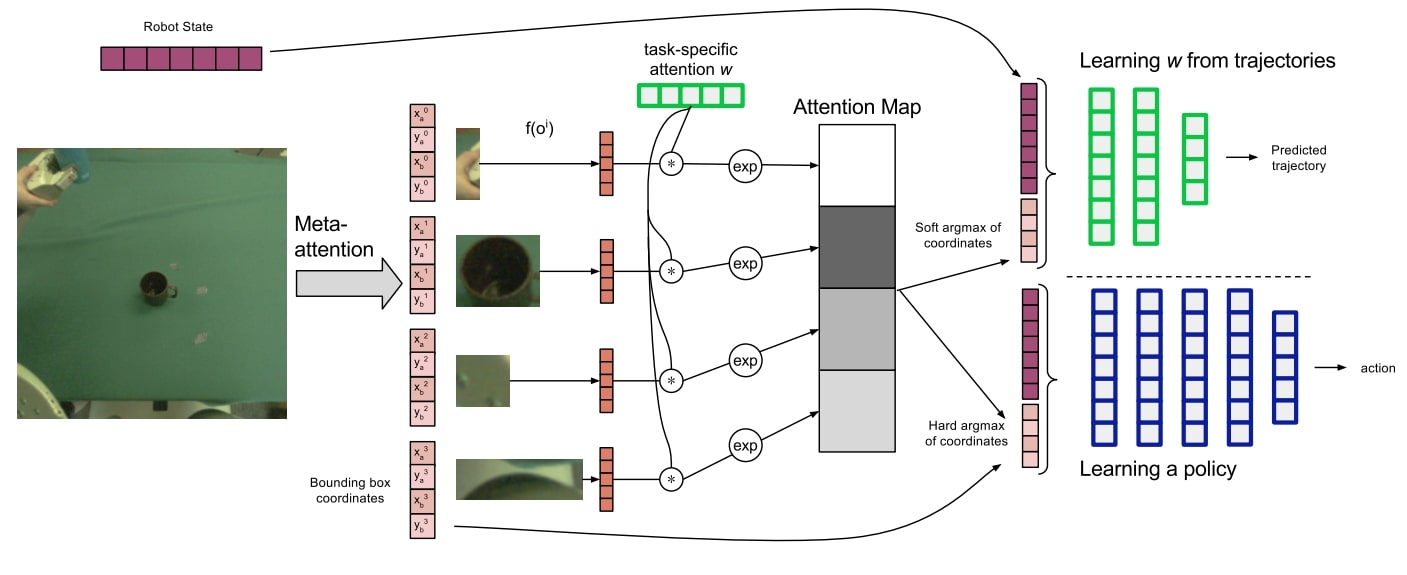
\includegraphics[width=0.8\textwidth]{figures/images/object_prior_framework.jpg}
    \caption{
            Robotic vision framework proposed in \cite{devin2018deep}. The framework is divided into different stages: \textbf{Meta-Attention}: Generates object proposals from an input image, trained on an object detection dataset, and shared across tasks; \textbf{Task-Specific Attention}: Focuses on relevant objects for a task using the meta-attention's semantic features; \textbf{Soft Attention}: Distributes attention as probabilities over object proposals using a Boltzmann distribution; \textbf{Movement Prediction Network}: Combines attended object information with the robot's state to predict the next action.
        }
    \label{fig:object_prior_framework}
\end{figure}